\documentclass[11pt]{article}
\usepackage[margin=1in]{geometry}
\usepackage{booktabs}
\usepackage{graphicx}
\usepackage{amsmath}
\usepackage{xcolor}
\usepackage{caption}
\usepackage[hidelinks]{hyperref}
\captionsetup{font=small,labelfont=bf}
\setlength{\parskip}{4pt}
\setlength{\parindent}{0pt}

\newcommand{\dsd}{DS\textsubscript{disrupted}}
\newcommand{\dsh}{DS\textsubscript{healthy}}
\newcommand{\hct}{HC\textsubscript{trust}}
\newcommand{\hce}{HC\textsubscript{equal}}

\title{\textbf{How Much of the Disruption Pile-Up Is a Routing Artifact?}\\
\large A deterministic routing-ladder study on the PSC simulator (no RL)}
\author{Aidan Hansen}
\date{June 9, 2026}

\begin{document}
\maketitle

\section*{Summary}
The $\sim$3{,}800-unit backlog that accumulates at the disrupted distributor was previously
treated as unavoidable (supply through the disrupted chain is capped at $\sim$20/period).
We tested that assumption by changing \emph{only the order-routing rules} --- no buffering, no
anticipation, no learning --- in a ladder of four configurations, scored at the
\textbf{system level} (all six agents) on held-out seeds.
\textbf{Result: roughly two-thirds of the during+post disruption cost is a routing artifact,
not physics.} Flipping the equal-split health center to trust-based splitting removes 26\%;
adding a sharper split rule and a stale-order write-off removes 67\%; adding an
onset-triggered reroute removes \textbf{91\%}. Under urgent demand, routing fixes alone
prevent 71--87\% of lost patients. During-disruption fill rate reaches 1.000: the healthy
chain could serve all demand all along --- the binding constraint was a routing rule, not
supply. This means our earlier value-decomposition numbers were computed against a hobbled
routing layer and must be recomputed, and the earlier ``detection captures $\approx$0'' claim
narrows to \emph{detect-then-buffer}: detect-then-\emph{reroute} is the single most valuable
deployable response measured to date.

\section{Question and motivation}

During the long disruption (periods 110--157), the manufacturer feeding \dsd{} drops to 5\%
capacity; deliveries through that chain are capped at $\sim$20/period against
$\sim$110/period of demand. Prior analysis concluded the resulting pile-up was unavoidable:
no ordering policy can pull more product through a capped chain.

That argument is correct \emph{given the routing configuration} --- but the configuration
contains two suspect rules, both verified in code. First, \hce{} splits its orders
\textbf{equally} between the two distributors by a fixed rule
(\texttt{decision\_maker.py:158}), so it keeps sending half its demand to the dead chain for
all 48 periods. Second, orders the dead chain cannot fill sit in the HC's \emph{on-order}
position indefinitely (no timeout), and the ordering formula subtracts on-order before
splitting (\texttt{decision\_maker.py:153}) --- so stranded orders also \textbf{suppress
re-ordering from the healthy chain}.

Why this gates the project framing: our earlier value decomposition attributed $-468$k to
``defending at all'' (a standing buffer) and $-654$k to ``timing'' (unreachable by
detection). If a large fraction of the disruption cost is recoverable by fixing a routing
rule, those numbers are conditional on a frozen routing layer, and the deployable-lever story
becomes three-fold: buffering, routing flexibility, and detection.

\section{Experimental setup}

\begin{table}[h]
\centering\small
\caption{Setup. All simulations are rule-based (base-stock ordering at every echelon); the
routing rule is the only thing that changes between rungs.}
\begin{tabular}{ll}
\toprule
\textbf{Component} & \textbf{Value} \\
\midrule
Topology & 2 MN $\to$ 2 DS $\to$ 2 HC; each HC dual-sourced from both DSs \\
Chains & MN1$\to$\dsd{}; MN2$\to$\dsh{} (no MN-level rerouting exists) \\
Demand (primary, urgent0) & non-urgent $\mathcal{N}(120,5)$ per HC per period; urgent $=0$ \\
Demand (secondary, urgent20) & non-urgent $\mathcal{N}(120,5)$; urgent $=20$ (lost if unmet) \\
Costs & holding 1/unit, backlog 10/unit, revenue 10/unit \\
Disruption & MN1 at 5\% capacity, periods 110--157 (48 of 300 periods) \\
Phases & pre 60--109, during 110--157, post 158--300 (warm-up excluded) \\
HC ordering & up-to $-$ on-order $-$ inventory $+$ backlog, capped at $\max(2d,120)$ \\
Trust & EMA of on-time delivery rate, $\delta=0.1$ \\
Seeds & \textbf{pre-registered}: tuning $=[1\text{--}10]$, reporting $=[11\text{--}30]$, paired \\
Scoring & \textbf{system-level} cost (all six agents), holding vs.\ backlog decomposed \\
\bottomrule
\end{tabular}
\end{table}

\begin{table}[h]
\centering\small
\caption{The routing ladder. Each rung adds one mechanism.}
\begin{tabular}{lp{11.5cm}}
\toprule
\textbf{Rung} & \textbf{Change} \\
\midrule
(a) & Baseline, exactly as configured in the repo: \hct{} splits by trust, \hce{} splits
      equally. Reproduces the prior base-stock reference bit-for-bit (gate 1). \\
(b) & \hce{} flipped to the same trust-based splitting \hct{} uses. The core test. \\
(c) & (b) $+$ sharper redirection (trust$^{4}$ split weights, trust update $\delta'=0.3$)
      $+$ \textbf{stale-order write-off}: on-order entries older than $5\times$ lead time are
      ignored by the ordering computation (accounting-only; the ledger is untouched, late
      deliveries still arrive and are costed honestly). Parameters tuned on tuning seeds
      only; the ranking was stable across the whole grid. \\
(d) & (b) $+$ oracle onset detection: from period 110 the HC split steps to a 90/10 share
      toward \dsh{}, reverting to trust dynamics after 157. This is
      \emph{detect-then-reroute} --- distinct from the \emph{detect-then-buffer} response
      that earlier analysis showed captures $\approx$0. \\
\bottomrule
\end{tabular}
\end{table}

Six verification gates passed before any reported number: (1) rung (a) under constant demand
reproduces the prior base-stock reference with \emph{zero} difference over 300 periods;
(2) per-seed determinism; (3) rung (b) measurably shifts \hce{}'s split; (4) the write-off
measurably reduces counted on-order; (5) per-period demand conservation at both HCs;
(6) cross-seed demand variation is nonzero. Gate 6 exists because we found
\texttt{NormalDistPatientModel.\_\_init\_\_} hard-resets the global RNG
(\texttt{patient\_model.py:28}), which had silently made every ``seed'' the same demand path
--- a finding that also affects any historical multi-seed result that used the normal demand
model. Our runner re-seeds after construction.

\section{Results}

\begin{table}[h]
\centering\small
\caption{Main results, urgent0 config, held-out reporting seeds 11--30 (mean over 20 seeds;
paired SEs are $\le 0.3\%$ of the mean everywhere, so they are omitted from the table).
TTR = time-to-recovery (periods after disruption end until \dsd{} backlog stays within 110\%
of its pre-disruption mean); AUB = area under the \dsd{} backlog curve, during+post
(threshold-free).}
\begin{tabular}{lrrrr}
\toprule
& \textbf{(a) baseline} & \textbf{(b) trust-split} & \textbf{(c) +sharp+w/o} & \textbf{(d) +onset} \\
\midrule
During+post system cost & 3{,}700{,}784 & 2{,}730{,}635 & 1{,}209{,}659 & 332{,}166 \\
\quad vs.\ baseline & --- & $\mathbf{-26.2\%}$ & $\mathbf{-67.3\%}$ & $\mathbf{-91.0\%}$ \\
\quad during / post & 2.58M / 1.13M & 2.10M / 0.63M & 0.95M / 0.26M & 0.20M / 0.14M \\
Pre system cost (sanity) & 17{,}044 & 17{,}040 & 17{,}045 & 17{,}040 \\
Peak backlog \dsd{} & 4{,}067 & 2{,}877 & 1{,}004 & 168 \\
Peak backlog \dsh{} & 139 & 199 & 572 & 528 \\
During fill rate (aggregate) & 0.808 & 0.897 & \textbf{1.000} & \textbf{1.000} \\
\quad \hct{} / \hce{} & 0.90 / 0.72 & 0.90 / 0.90 & 1.00 / 1.00 & 1.00 / 1.00 \\
TTR \dsd{} (periods) & 18 & 13 & 7 & 38.9$^{\dagger}$ \\
AUB \dsd{}, during+post & 131{,}253 & 93{,}526 & 33{,}797 & 4{,}126 \\
\midrule
\multicolumn{5}{l}{\emph{urgent20 config (same seeds):}} \\
During+post system cost & 3{,}908{,}652 & 2{,}865{,}974 & 1{,}339{,}087 & 447{,}451 \\
Lost patients (episode) & 1{,}768 & 1{,}594 & \textbf{510} & \textbf{236} \\
\quad vs.\ baseline & --- & $-10\%$ & $\mathbf{-71\%}$ & $\mathbf{-87\%}$ \\
\bottomrule
\multicolumn{5}{p{14.5cm}}{\footnotesize $^{\dagger}$The 110\%-threshold misbehaves for (d):
its pre-disruption backlog is $\approx 0$, so the threshold is tiny and the rung is penalized
for clearing a small residual slowly. The threshold-free AUB row is the honest comparison.}
\end{tabular}
\end{table}

\begin{figure}[h]
\centering
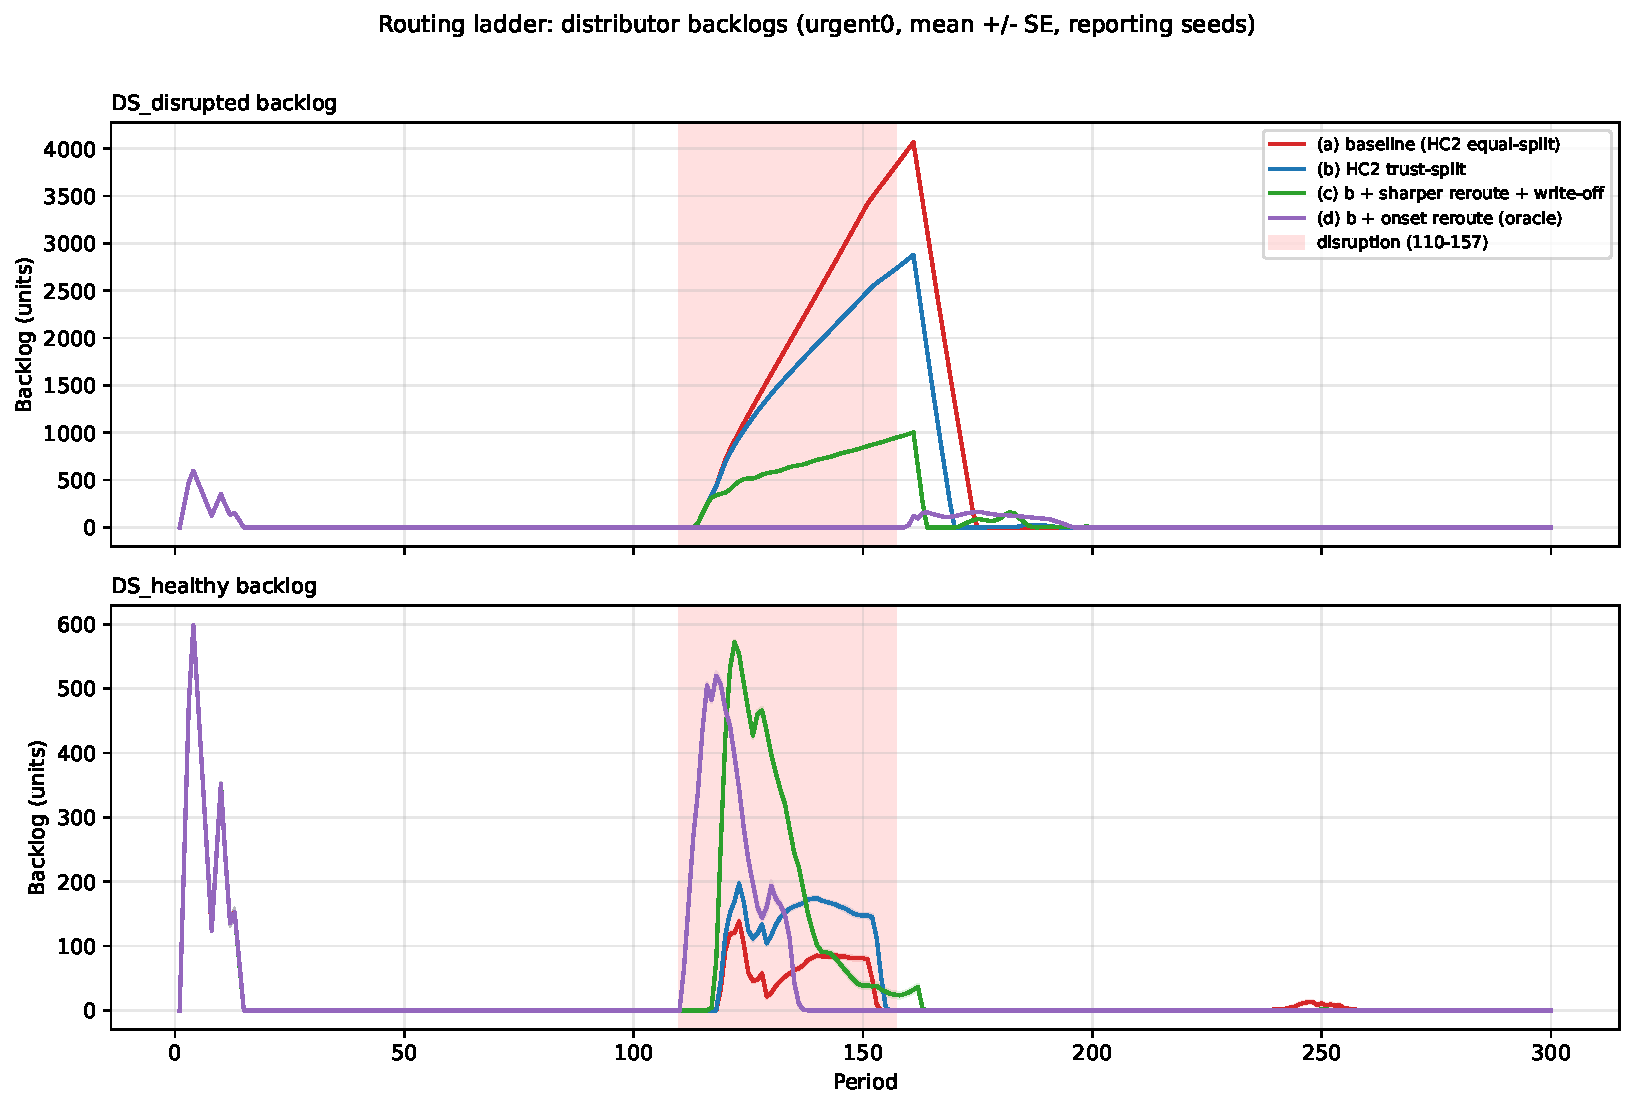
\includegraphics[width=0.93\textwidth]{../results/figures/backlog_trajectories_urgent0.pdf}
\caption{Distributor backlogs by rung (urgent0, mean $\pm$ SE over reporting seeds). The
baseline pile-up at \dsd{} (top, red) shrinks rung by rung; \dsh{} (bottom; note the
$6\times$ smaller scale) absorbs the redirected demand with only a brief transient ---
no mirror-image pile-up forms.}
\end{figure}

\begin{figure}[h]
\centering
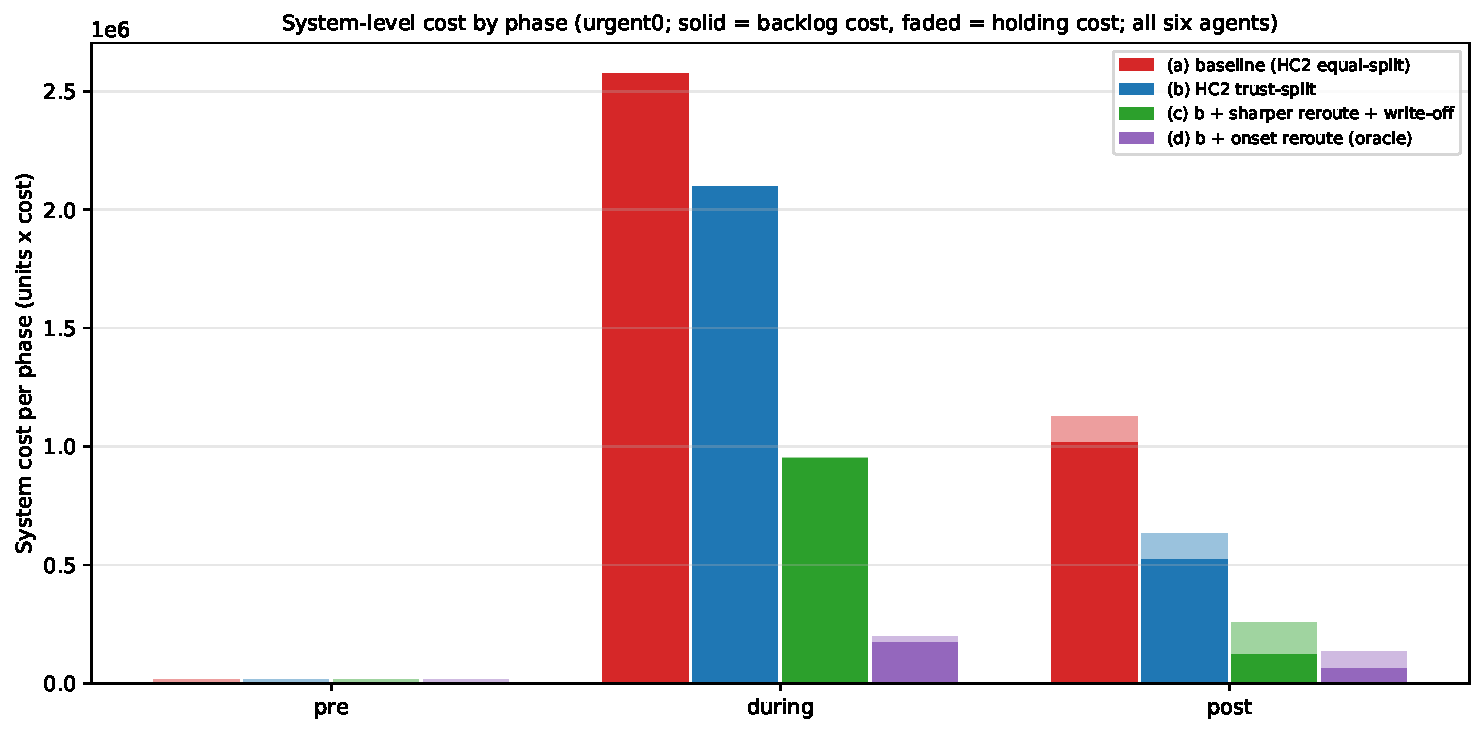
\includegraphics[width=0.9\textwidth]{../results/figures/cost_by_phase_urgent0.pdf}
\caption{System-level cost by phase (solid = backlog cost, faded = holding cost, all six
agents). Pre-phase costs are identical across rungs (no rung does anything before the
disruption); the entire effect is during+post. Rung (c)'s slightly higher post holding is
the write-off's late-delivery glut, honestly costed and dwarfed by its backlog savings.}
\end{figure}

\begin{figure}[h]
\centering
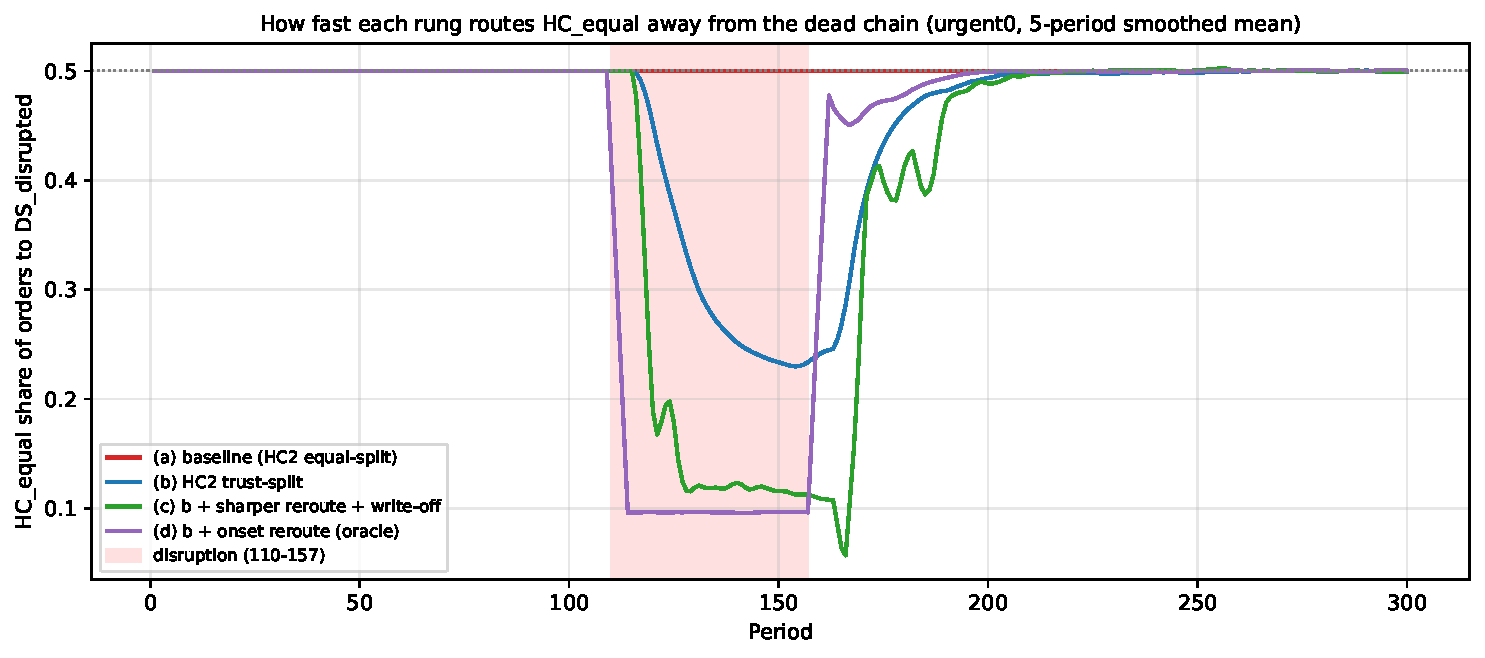
\includegraphics[width=0.9\textwidth]{../results/figures/split_share_urgent0.pdf}
\caption{The mechanism, directly: \hce{}'s share of orders sent to the dead chain. Baseline
(red) stays at 0.5 by rule. Plain trust-split (blue) redirects slowly and bottoms out at
$\sim$0.23 --- the trust-EMA floor predicted in the hypothesis doc. The sharper rule (green)
reaches $\sim$0.12 within $\sim$10 periods; the onset reroute (purple) steps there
immediately. All revert after recovery.}
\end{figure}

\clearpage
\section{Interpretation and caveats}

\textbf{The healthy chain could serve everything all along.} Under rungs (c)/(d) the
during-disruption fill rate is 1.000: MN2 (capacity 400/period, normally loaded $\sim$120)
absorbs all redirected demand. The system was never supply-capped --- only the disrupted
\emph{chain} was. ``The pile-up is unavoidable'' was true only chain-locally.

\textbf{Each mechanism contributes measurably.} Equal-split lock-in costs 26\%; trust's slow,
incomplete redirection plus stranded-order suppression another 41 points; detection timing
the last 24. The fairness effect is also fixed: baseline harm concentrates on \hce{}
(fill 0.72 vs.\ 0.90), and every fixed rung equalizes the HCs.

\textbf{What this means for our earlier numbers.} The value decomposition
($-468$k buffer / $-654$k timing) was measured with the routing layer frozen in its hobbled
state; it must be recomputed on a routing-fixed baseline. The ``detection captures
$\approx$0'' result was real but response-specific: buffering a supply-capped chain
post-onset is futile, while rerouting demand post-onset is worth $\sim$0.88M (the c$\to$d
gap) plus half of rung (c)'s remaining lost patients. The \emph{anticipation} impossibility
result stands untouched: nothing is observable before period 110, and rung (d) uses an
oracle onset signal, so (d) is an upper bound on real detect-then-reroute. Since (c) reaches
the redirected state within $\sim$10 periods with no detector at all, a real detector with a
few periods of latency lands between (c) and (d).

\textbf{Caveats.} The Doroudi et al.\ (2020) non-monotonicity prior (trust-sensitive buyers
can be \emph{disadvantaged} in some regimes) did not bind here --- rung (b) improved every
metric --- but we tested one disruption regime; severity/duration robustness is queued.
Results are one topology (2$\times$2$\times$2, healthy chain has ample headroom); in a regime
where the healthy chain \emph{cannot} absorb total demand, buffering should re-emerge as the
binding lever. Rung (c)'s parameters were tuned on separate seeds, and the tuning ranking was
stable, but the rule forms (trust$^{p}$, age write-off) were chosen by us, not optimized over
rule space.

\section{Next steps and future directions: simple heuristic policies}

The following is assessment, not measured result, except where numbers are cited.

\textbf{Immediate next experiments (all deterministic, unblocked):}
\begin{enumerate}
\item \textbf{Recompute the value decomposition on the rung-(c) baseline} --- rerun the buffer
sweep and clairvoyant ceiling with routing fixed. This replaces the $-468$k/$-654$k numbers
and decides how much room is left for \emph{any} anticipatory policy. Highest priority.
\item \textbf{Real detector in rung (d)} --- swap the oracle for the delivery-shortfall
detector from the earlier detection study; measure what detection latency costs against the
(c)--(d) gap.
\item \textbf{Buffer $\times$ routing interaction} --- $\{$no buffer, always-defend$\}\times
\{$rung a, rung c$\}$: is buffering still worth anything once routing is fixed? (Prediction:
little, at this severity --- fill rate is already 1.000 under (c).)
\item \textbf{Robustness} --- short/moderate disruptions, 50--80\% capacity cuts, and a
severity where \dsh{} \emph{cannot} absorb everything.
\end{enumerate}

\textbf{Which simple heuristics look promising (for the heuristic-frontier paper):}
\begin{itemize}
\item \textbf{Trust-sharpening (trust$^{p}$) and faster trust updates} --- two-line change,
no detection, captured $-41$ points here. The single best value-per-complexity lever found
so far.
\item \textbf{Stale-order write-off (age $> k\times$ lead time)} --- deployable accounting
rule; in real supply chains this is just order-expiry. Part of the same $-41$ points.
\item \textbf{Detect-then-reroute} --- the one detection-based policy with measured value.
Pairs a trivial onset detector (delivery shortfall) with a demand-side response.
\item \textbf{Post-disruption catch-up throttle} --- cap the order rate while clearing
backlog, to suppress the recovery glut (visible in rung (c)'s post holding). Untested;
cheap to add to the ladder.
\item \textbf{Serve-captive allocation at the disrupted DS} --- with routing fixed, the
disrupted DS's trickle should arguably go to whichever HC remains stuck with it. Tests
dossier Mechanism 3 without any RL.
\item \textbf{Permanent buffer} --- now demoted to the lever of last resort for regimes where
the healthy chain lacks headroom; its standing holding cost only pays off where routing
cannot.
\end{itemize}

For the eventual RL comparison, this study sharpens the bounding-paper structure: simple
rules now occupy $-67\%$ (no detection) to $-91\%$ (oracle detection) of the achievable
range, so any learned policy must be evaluated against the rung-(c) baseline, not against
the broken-routing baseline --- and the residual available to learning is the gap between
rung (c) and the (to-be-recomputed) clairvoyant ceiling.

\end{document}
